\begin{tcolorbox}[colbacktitle=gray, title={\fontsize{35pt}{0pt}\selectfont 特徴探索}]
	\structure{探索空間} \\
	\vspace{80pt}\\
	全部分グラフを列挙するような\\
	\vspace{10pt}\\
	木状の探索空間(gspan木)\\
	\vspace{30pt}\\
	$~~ \rightarrow$ DAG状探索空間に拡張
	\begin{textblock*}{\textwidth}(230pt,-220pt)
		\begin{figure}[h]
			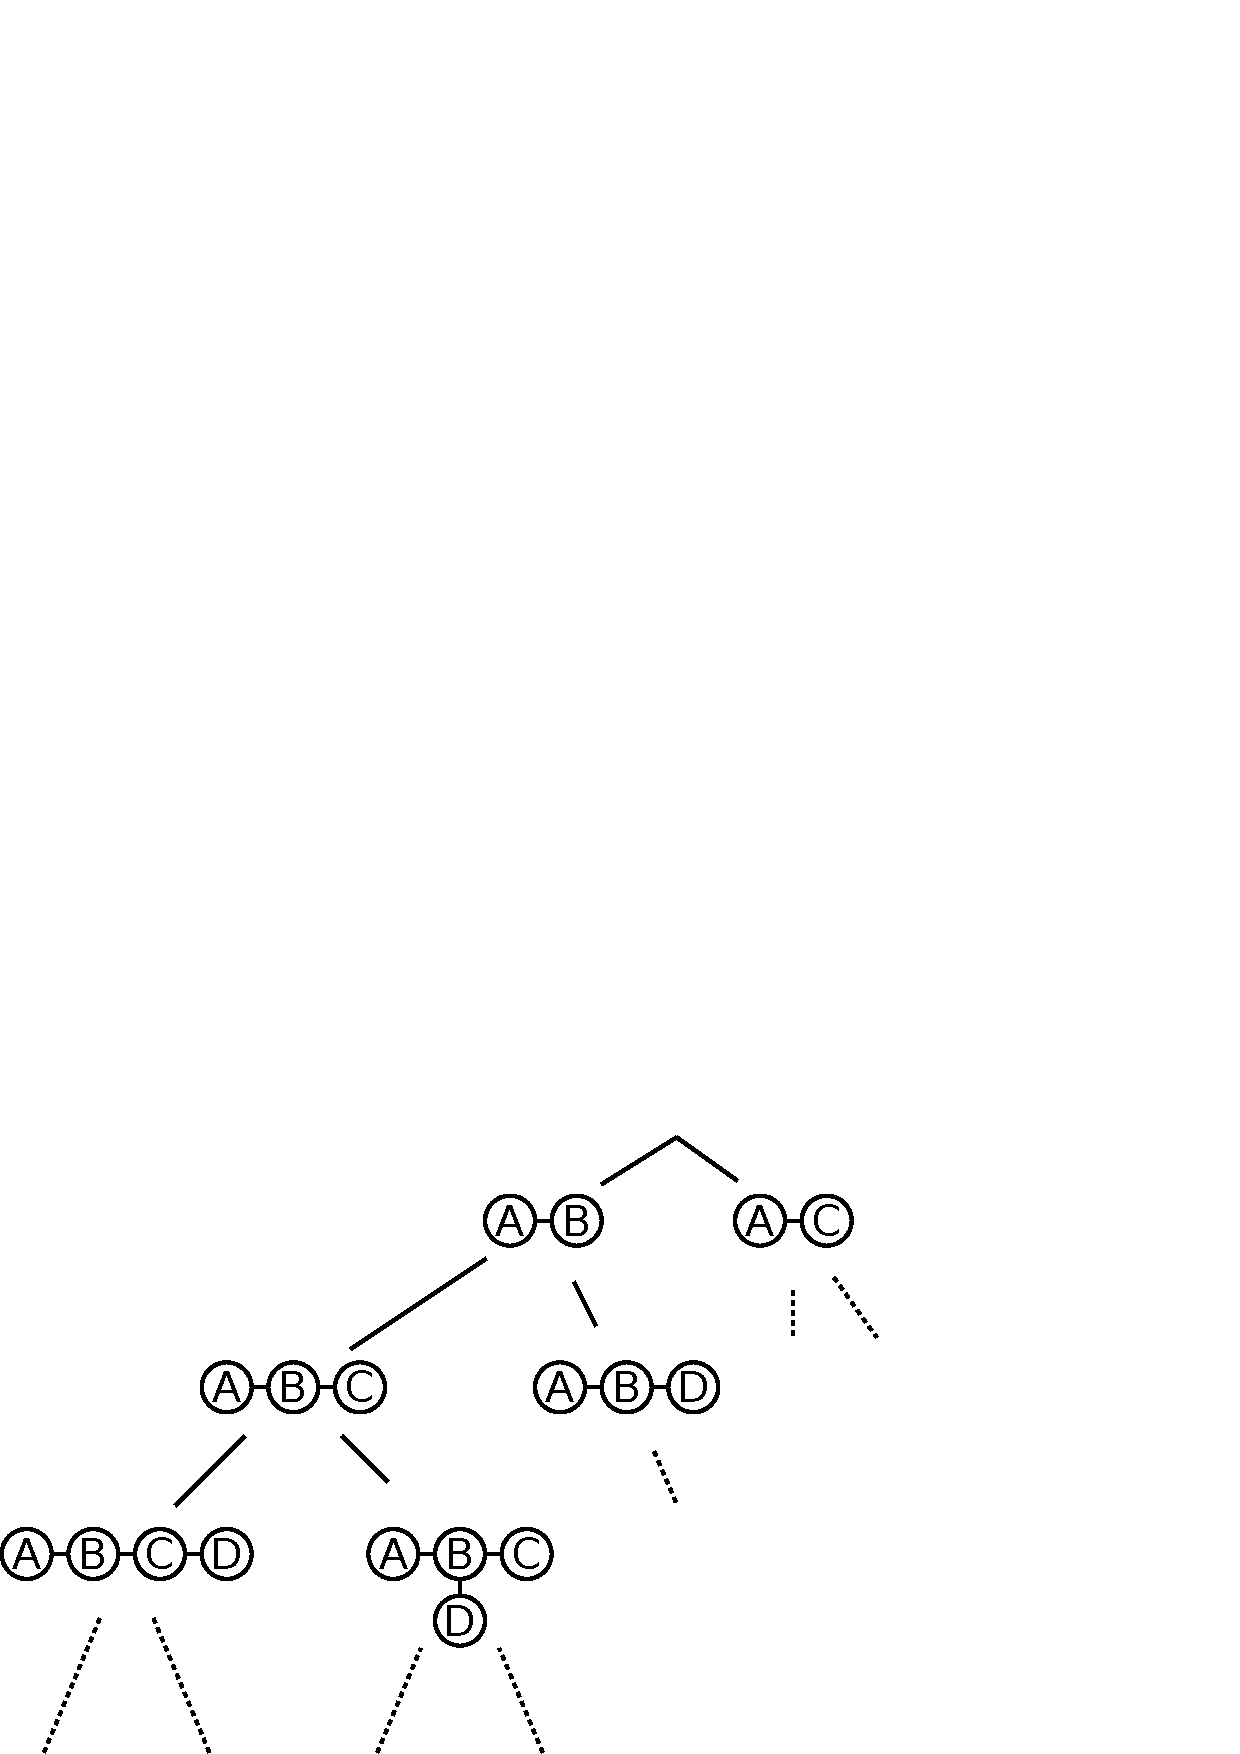
\includegraphics[width=0.42\hsize]{img/graph_search_tree.png} \\
			\vspace{5pt}
			DAG状空間
		\end{figure}
	\end{textblock*}
	
	\vspace{150pt}
	\structure{モンテカルロ木探索} \\
	\vspace{10pt}\\
	UCTアルゴリズムを利用した特徴探索により探索コストを削減
	\vspace{50pt}\\
	UCTアルゴリズムにおける4操作
	\vspace{20pt}

	\begin{easylist}[itemize]
		@ Selection
		\vspace{10pt}
	\end{easylist}
	\hspace*{60pt}
	根ノードからUCB(Upper Confidence Bound)の値をもとに\\
	\hspace*{60pt}
	探索済みノードの末端まで子ノードを選択
	\begin{align*}
		\argmax_{c_{j} \in \{\mbox{\fontsize{22pt}{0pt}子ノード集合}\} }\ UCB,
		\hspace*{60pt}
		UCB = \bar{V} + C \sqrt{2 \frac{logN}{n_{j}}}
	\end{align*}
	\begin{align*}
		\bar{V}:c_{j}\mbox{\fontsize{22pt}{0pt}の選択による報酬平均},
		\ C:\mbox{\fontsize{22pt}{0pt}探索強度パラメータ}, 
	\end{align*}
	\begin{align*}
		\ N:\mbox{\fontsize{22pt}{0pt}親ノードの選択回数},
		\ n_{j}:c_{j}\mbox{\fontsize{22pt}{0pt}の選択回数}
	\end{align*}
	\begin{align*}
		\mbox{※}\ \fontsize{22pt}{0pt}{\mbox{報酬} = - [\TSS(D_1(x_j)) + \TSS(D_0(x_j))]}
	\end{align*}

	\vspace{30pt}
	\begin{easylist}[itemize]
		@ Expansion
		\vspace{10pt}
	\end{easylist}
	\hspace*{60pt}
	末端ノードの選択回数が閾値を越えた場合に、\\
	\vspace{10pt}\\
	\hspace*{60pt}
	その末端ノードの子ノードを探索空間に追加する

	\vspace{40pt}
	\begin{easylist}[itemize]
		@ Simulation
		\vspace{10pt}
	\end{easylist}
	\hspace*{60pt}
	選択された末端ノードパターンを拡大する \\
	\vspace{10pt}\\
	\hspace*{60pt}
	停止条件:確率的停止 or 拡大不可

	\vspace{40pt}
	\begin{easylist}[itemize]
		@ Backpropagation
		\vspace{10pt}
	\end{easylist}
	\hspace*{60pt}
	Simulationによって拡大されたノードパターンに対して報酬を計算\\
	\vspace{10pt}\\
	\hspace*{60pt}
	$~~ \rightarrow$ 辿ったパスのUCB値を更新

	\vspace{80pt}
	\fontsize{34pt}{0pt} \selectfont
	有望な空間をより深く探索\\
	\vspace{10pt}\\
	$~~ \rightarrow$ 制限されたコスト内でより良い解の発見
\end{tcolorbox}
